\documentclass[a4paper]{article}

%=======================================================================

\usepackage[authoryear, round]{natbib}
\usepackage{url}
\usepackage[intlimits]{amsmath}
\usepackage{amssymb}
\usepackage{graphicx}

%=======================================================================

%============================================================
% Roman Characters
%============================================================

% differential d
\newcommand{\dd}{{\rm d}}

% Euler's number
\newcommand{\rme}{{\rm e}}

%============================================================
% Misc.
%============================================================

% margins of a proper size
\let\oldmarginpar\marginpar
\setlength{\marginparwidth}{3cm}
\renewcommand\marginpar[1]{%
  \oldmarginpar[\raggedleft\footnotesize #1]%
  {\raggedright\footnotesize #1}%
}

% average
\newcommand{\ave}{\braket}

% vectors
\newcommand{\vect}[1]{\boldsymbol{#1}}

% partial derivative
\newcommand{\pder}[2]{\frac{\partial {#1}}{\partial {#2}}}


%=======================================================================

\title{Shallow water model}
\author{Martin Claus, Willi Rath}
\date{\today}

%=======================================================================

\begin{document}

\maketitle

%=======================================================================

\section{Equations}

In Cartesian coordinates, the system is described by
\begin{align}
  & u_t - fv = -g \eta_x + F^x \\
  & v_t + fu = -g \eta_y + F^y \\
  & \eta_t + (Hu)_x + (Hv)_y = 0
\end{align}
Spherical coordinates with $a$ being the radius of the earth, $\lambda$ the 
longitude, and $\vartheta$ the latitude:
\begin{align}
  & u_t - fv = -g \frac{1}{a\cos\vartheta}\pder{\eta}{\lambda} + F^x \\
  & v_t + fu = -g \frac{1}{a}\pder{\eta}{\vartheta} + F^y \\
  & \eta_t + \frac{1}{a\cos\vartheta}\pder{Hu}{\lambda} + \frac{1}{a\cos\vartheta}\pder{\cos\vartheta Hv}{\vartheta} = 0
\end{align}

%=======================================================================

\section{Grid}

We want the grid to be as natural as possible (i.e., no averaging in the 
$\eta$-gradients and in the continuity equation):

\begin{figure}[h]
  \begin{center}
    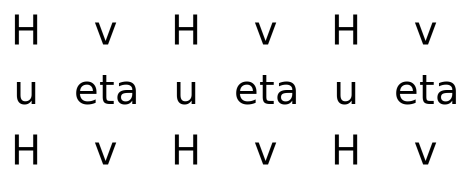
\includegraphics[width=0.35\textwidth]{images/grid}
  \end{center}
  \caption{Grid arrangement. We use an Arakawa C-grid with the topography
    on the free grid points.  }
\end{figure}

The fields will all carry integer indices which are to be interpreted according to
\begin{align}
  H|_H^{ij} & = H(\Delta x \cdot i, \Delta y \cdot j) \\
  \eta|_\eta^{ijl} & = \eta(\Delta x \cdot (i+1/2), \Delta y \cdot (j+1/2), \Delta t \cdot l) \\
  u|_u^{ijl} & = u(\Delta x \cdot i, \Delta y \cdot (j+1/2), \Delta t \cdot l) \\
  v|_v^{ijl} & = v(\Delta x \cdot (i+1/2), \Delta y \cdot j, \Delta t \cdot l)
\end{align}
An expression like $H|_u^{ij}$ means that the depth is interpolated to the $u$-grid
by simple linear interpolation which is two-point averaging here. In the Coriolis term, 
we'll need four point averaging from the $v$-grid to the $u$-grid and from the $u$-grid
to the $v$-grid. The $x$- and $y$-derivatives in the continuity equation will all need 
two point averaging from the $H$-grid to the $u$- and $v$-grid.

%=======================================================================

\section{Boundary conditions}

%-----------------------------------------------------------------------

\subsection{Coastlines / Land mask}

We'll define land to be where $H$ is zero. This implies that $u$- and $v$-grid
points are over land if both the closest $H$-grid points are over land.
$\eta$-grid points are over land, if all four surrounding $H$-grid points are over land.
It will probably be computationally effective to define masks for all three dynamic variables.

%-----------------------------------------------------------------------

\subsection{Periodic boundary conditions}

For a global model, we'll need to implement periodic boundary conditions in the zonal
direction.  In the meridional direction we might get away without as we won't be able 
to extend the model domain to the poles anyway (CFL will become a problem there).

%=======================================================================

\section{Time stepping scheme}

Use Heaps (1972) which basically amounts to\footnote{Note that the superscrip
of $v$ in the second equation is mean to be an $l$ while all the others are meant
to be $l+1$. In each line, you use the newest information that is available ...}
\begin{align}
  \eta^{l+1} & = \eta^l - \Delta t (Hu^l)_x - \Delta t (Hv^l)_y \\
  u^{l+1} & = u^l + \Delta t f v^l - \Delta t g \eta^{l+1}_x \\
  v^{l+1} & = v^l - \Delta t f u^{l+1} - \Delta t g \eta^{l+1}_y
\end{align}

Spherical coordinates with full\footnote{There still is an implicit two point
averaging from the $H$-grid to the $u$- and $v$-grids as well as an implicit
four point averaging in the Coriolis term.} glory:
\begin{equation}
  \begin{split}
    \eta|_\eta^{i,j,l+1} & = \eta|_\eta^{ijl} \\
    & \quad - \frac{\Delta t}{a\cos\vartheta|_\eta^{j}\Delta\lambda}
      \Biggl(H|_u^{i+1,j} u|_u^{i+1,j,l} - H|_u^{ij}u|_u^{ijl}\Biggr) \\
    & \quad - \frac{\Delta t}{a\cos\vartheta|_\eta^{j}\Delta\vartheta}  
      \Biggl(H|_v^{i,j+1}\cos\vartheta|_v^{j+1}v|_v^{i,j+1,l} - H|_v^{ij}\cos\vartheta|_v^{j}v|_v^{ijl}\Biggr)
  \end{split}
\end{equation}

\begin{equation}
  u|_u^{i,j,l+1} = u|_u^{ijl} 
    + \Delta t f v|_u^{ijl}
    - \frac{\Delta t g}{a\cos\vartheta|_u^j\Delta\lambda}
      \Biggl(\eta|_\eta^{i,j,l+1} - \eta|_\eta^{i-1,j,l+1}\Biggr)
\end{equation}

\begin{equation}
  v|_v^{i,j,l+1} = v|_v^{ijl} 
    - \Delta t f u|_v^{i,j,l+1} 
    - \frac{\Delta t g}{a\Delta\vartheta}
      \Biggl(\eta|_\eta^{i,j,l+1} - \eta|_\eta^{i,j-1,l+1}\Biggr)
\end{equation}

In the model, we'll calculate $H|_u^{ij}$ and $H|_v^{ij}$ once in the beginning and
then use it throughout the simulation. However, for defining which grid points are 
over land, it is still helpful to use the original $H$-grid.

%=======================================================================

\section{Stability}

Note that we will not consider optimization of roundoff errors at this point. We'll stick
to SI-units and readable code as long as possible.

There are two criteria which may be of importance: $|\Delta t\cdot f|<1$ which comes from the
Coriolis term, and the CFL criterion $c\frac{\Delta t}{\Delta x}=\sqrt{gH}\frac{\Delta t}{\Delta x}<1$. The CFL
criterion is by far the most dangerous. From the first criterion, $\Delta t$ varies from infinity
at the equator to half a day at the poles, while from CFL with high resolution, high latitudes and 
large $H$ time steps of much less than $10$ seconds can easily arise.
\begin{equation}
  \Delta t < \frac{\Delta\lambda/deg \cdot 111km \cdot \cos\vartheta^{max}}{\sqrt{gH}} 
\end{equation}
For $H=O(10km)$, $\Delta\lambda=1/10^{o}$ and a model domain which extends up to $89N$, this results in 
as short a time steps as $0.6$ seconds.

%=======================================================================

\section{Estimation of computational effort}

In the end, we might want to simulate an almost global model 
(say $\lambda=0\ldots360^o$, $\vartheta=-89\ldots89^o$) with a resolution 
of up to $1/10^o$ for more than one year of model time. There are 
$360*178*100\approx 6.5\cdot10^6$ grid points and for each grid point we need $O(20)$ 
multiplications and additions. The time step is $\approx 0.6s$ and one year of model time
has $\approx 3.15\cdot 10^7s$. Altogether, we need $N\approx 6.7\cdot 10^{15}$ operations which
on a machine with $8GFLOPS$ can be done in $8.5\cdot 10^5s\approx 10d$. For a smaller domain, which
only extends to $85^o$ in latitude, only about $2d$ are necessary.

%=======================================================================

\section{First test: Rectangular domain}

Domain:
\begin{equation}
  \begin{split}
    \lambda & = -20^o \ldots 20^o \\
    \vartheta & = -20^o \ldots 20^o \\
    \Delta \lambda & = \Delta \vartheta = 0.4^o \\
    H & = 1000m = const. \\
    \Rightarrow \Delta t & = 422 s \\
  \end{split}
\end{equation}

Initial conditions:

Adjustment should be done after $O(20 \cdot 2 \cdot 111km / \sqrt{gH}) = 
O(4.5\cdot 10^4s) = O(100) \Delta t$.

%=======================================================================

%\bibliographystyle{plainnat}
%\bibliography{bibliography}

\end{document}
